%%%%%%%%%%%%%%%%%%%%%%%%%%%%%%%%%%%%%%%%%%%%%%%%%%%%%%%%%%%%%%%%%%%%%%%%%
%
% This file defines the style for your homebook
% You don't need to edit it any more, if not to 
% change the authors name:
%
% Search below for the keyword:   GROUP
% insert your group number
%
% Search below for the keyword:   AUTHORS
% insert the name of the authors
%
%%%%%%
% Now to update the dexcription  of your work you will 
% use the file ``master.tex'' in the current directory
% following the instructions in it 
%
%%%%%% 
%%%%%%  
%%%%%%
% If you want to compile your document you have TWO ways
% depending on the fact that 
% 	1) you have inserted only postcript images in your tex file 
%		---> then go to MODE 1
%	2) you have inserted other kind of images (jpg..) in your tec file
%		---> then go to MODE 2
%
% MODE 1 
%simple type:
% 	latex homebook.tex
%
% If the compilation runs succesfully and you want to see the results type:
% 	xdvi homebook.dvi &
% and use the menus to go through the document
%
% If you want to create a pdf type:
% 	dvipdfm homebook.dvi
%
% a homebook.pdf file is created
% you can see it using the command:
% 	acroread homebook.pdf &
%
%
% MODE 2
% simple type:
%	pdflatex homebook.tex
%
% If the compilation runs succesfully you directly have the pdf file
% and you can see it using the command:
%       acroread homebook.pdf &
%
% 
%%%%%%%%%%%%%%%%%%%%%%%%%%%%%%%%%%%%%%%%%%%%%%%%%%%%%%%%%%%%%%%%%%%%%%%%%%
\documentclass[10pt,  english, makeidx, a4paper, titlepage, oneside]{book}
\usepackage{babel}
\usepackage{fancyhdr}
\usepackage{fancyvrb}
\usepackage{makeidx}
\usepackage{titlesec}
\usepackage{listings} 
\usepackage{hyperref}


\newenvironment{listato}{\footnotesize}
                        {\normalsize }


%\pagestyle{empty}

\textwidth 15.5cm
\textheight 23cm
\topmargin -1cm
\oddsidemargin -0.5cm
\linespread{1.1}

\pagestyle{fancy}
\lhead{}
\chead{Integrated Systems Architecture}
\lfoot{}
\cfoot{}
\rfoot{}
\rhead{\thepage}

\usepackage{graphicx}
\usepackage{amsmath}
\usepackage{amsfonts}
\usepackage{amsthm}
\usepackage{amssymb}
%\oddsidemargin -1.1cm

\titleformat{\chapter}[display]
{\normalfont\Large\filcenter\sffamily}
{\titlerule[0.5pt]%
\vspace{1pt}
\titlerule
\vspace{1pc}
\LARGE\MakeUppercase{\chaptertitlename} \thechapter
}
{1pc}
{\titlerule
\vspace{1pc}
\Huge}

\newcommand{\SubSubSection}[1]{\subsubsection{\bf Exercise   ~#1}}

\newcommand{\homework}[1]{\subsubsection{\bf Homework   ~#1}}

\newcommand{\Solution}{\subsubsection{\bf Solution}}




\makeindex
\begin{document}
\frontmatter
\begin{titlepage}
\vspace{2cm}
\centerline{

\includegraphics[width=2cm]{./logopoli}}  
\centerline{\LARGE Politecnico di Torino}
\bigskip
\centerline{\Large III Facolt\`a di Ingegneria}
\vspace{4cm}
\centerline{\Huge\sf Lab 1 Report}
\bigskip
\centerline{\Huge\bfseries\sf Integrated Systems Architecture}
\vspace{2cm}
\centerline{\LARGE Master degree in Computer Engineering}
\vspace{4.4cm}
%%%%%%%%%%%%%%%%%%%%%%%%%%%%%%%%%%%%%%%%%%%%%%%%%%%%%%%
% GROUP
% Change the name of your group below
%
\centerline{\Large Authors: ISA36}
\vspace{2cm}
%
%%%%%%%%%%%%%%%%%%%%%%%%%%%%%%%%%%%%%%%%%%%%%%%%%%%%%%%
% AUTHORS
% Change the name of the Group participants here
%
\centerline{Nicole Dai Pr\`a s274501, Leonardo Izzi s278564}
%
%%%%%%%%%%%%%%%%%%%%%%%%%%%%%%%%%%%%%%%%%%%%%%%%%%%%%%
\vspace{2cm}
\centerline{\today}
\vspace{1cm}
{\scriptsize Many thanks to Prof. Mariagrazia Graziano for providing us with this template.}
\end{titlepage}

\tableofcontents

%%%%%%%%%%%%%%%%%%%%%%%%%%%
% 
\mainmatter
\lstset{language=VHDL}

%%%%%%%%%%%%%%%%%%%%%%%%%%%%%%%%%%%%%
%%%%%%%%%%%%%%%%%%%%%%%%%%%%%%%%%%%%%
%%    
%% HERE IS THE MAIN INCLUSION
%%
\chapter{Introduction}

In this laboratory session we have learned the principles behind UVM and how to test both combinational and sequential circuits.
As required, there is a GitHub repository available at the following link: \url{https://github.com/leoizzi/isa_labs/tree/main/lab4}.

There are three top folders, which are:
\begin{itemize}
    \item \verb|adder|, where the test of the given adder has been performed.
    \item \verb|fpmult|, where the test of the whole floating point multiplier has been performed.
    \item \verb|mult|, where the test of the MBE-Dadda tree multiplier has been performed.
\end{itemize}

Each of these folders has the same structure, which is:
\begin{itemize}
    \item \verb|sim|, the folder containing all the transcripts produced by QuestaSim.
    \item \verb|src|, the folder containing the files related to the DUT.
    \item \verb|tb|, the folder containing all the files related to the verification.
\end{itemize}
\chapter{IIR}
\label{chap:iir}

In this chapter the IIR filter is analyzed from its Matlab specification to the physical design.

\section{Matlab model}

We have updated \verb|my_iir_filter.m| to match the value of the given $N$ and $n_{b}$ values.
This file saves the quantized filter's input in a file called \verb|samples.txt|, which is then used
by the C model (section \ref{sec:iir_c_model}) to test the goodness of the implementation.
After the C model's simulation, its results are read back to measure the {\it Total Harmonic Distortion}
($THD$). By keeping the internal representation on 12 bits we have measured $THD \approx -65.46\ dB$, which is
better than $THD_{target} = -30\ dB$, hence the whole filter has been implemented on 12 bits.


\section{C model}
\label{sec:iir_c_model}

In the C model we have only modified the coefficients to match the ones given by Matlab and the shift amount,
because a shift of \verb|NB-1| in our case resulted in an internal representation of 13 bits, while as said
earlier 12 bits were enough. Therefore, we have added a macro called \verb|INT_REPR| set to 1 which is
added to the previous term to obtain the target shift value. The output values have been stored in a file
called \verb|results_c_12bit.txt|.

\section{VHDL model}

\begin{figure}[!ht]
	\centering
	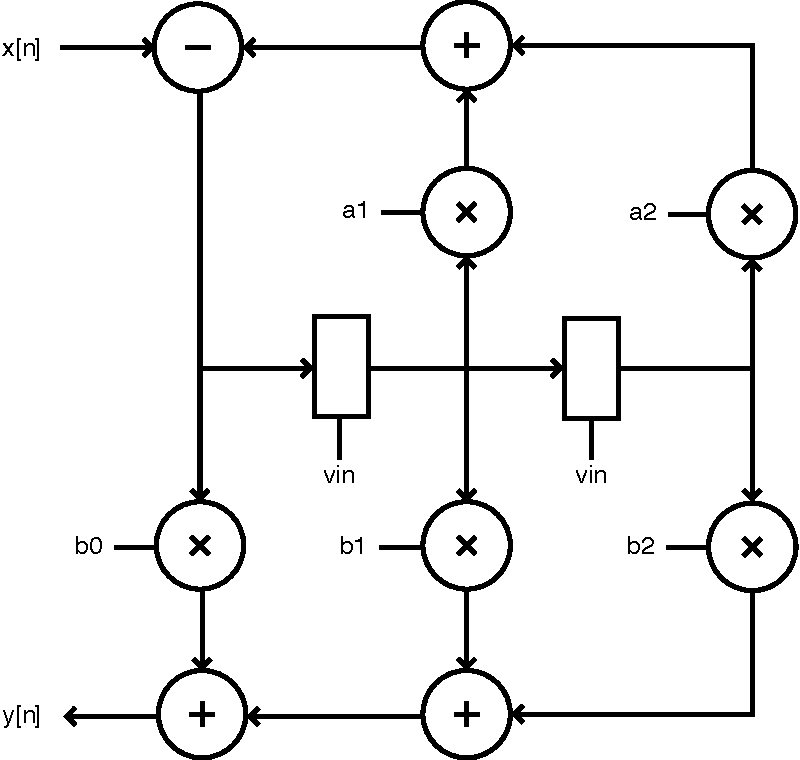
\includegraphics[width=0.4\linewidth]{./chapters/pictures/iir.pdf}
	\caption{IIR direct form II block diagram}
	\label{fig:iir}
\end{figure}

The filter has been implemented by deriving its structure from the C model and by using behavioral, generic components
for the arithmetic operations. The top module, instead, is not generic and its implemented in a structural way. It is
contained in the file \verb|iir.vhd|. In figure \ref{fig:iir} is shown the block diagram of the IIR.

The model entirely reflects the one described in C as it can be seen, the only peculiarity is in the organization of the
register's enable signals, not shown in picture \ref{fig:iir} (along with the input, coefficients and output registers)
to reduce the clutter.
Since the structure is so small no control unit has been developed. Instead, we have decided to add 1 bit registers to
store the delayed value of vin to correctly drive the filter.
The \verb|x[n]| register, along with the ones shown in the figure (that correspond to the C model's sw[i] array) and the
coefficients' registers are enabled by \verb|vin| itself. \verb|y[n]| register, on the other hand, takes as enable \verb|vin|
delayed by 1 clock cycle since it has to latch the value computed the cycle before. This means that the value of y[n] is
available to the filter's interface only the cycle after the register have been enabled, so the signal \verb|vout| corresponds
to \verb|vin| delayed by 2 clock cycles.

\subsection{Simulation}

This circuit has been simulated with {\it ModelSim}, that has written the simulation result in a file called
\verb|results_vhdl_12bit.txt|. The \verb|diff| tool has been run on the C model's output and this file to check that the
VHDL model was compliant with it.
To reproduce the simulation there is a script in the \verb|sim| folder called \verb|sim_script.tcl|.

\subsection{Logic synthesis}

The model described above has been synthesized with {\it Synopsys Design Compiler}. The synthesis has been run three times:

\begin{itemize}
    \item \textbf{Run 1}: to find the maximum clock frequency we have created a clock with period 0 with the command \verb|create_clock -name my_clk -period 0 clk|. With \verb|report_timing| we have found out that $t_{ck_{min}} = 2.81\ ns$.
    \item \textbf{Run 2}: to verify that $t_{ck_{min}}$ was actually a valid value we run a synthesis with a clock period $t_{ck} = t_{ck_{min}}$. The synthesis met the constraint and the area for this implementation is $A_{ck_{min}} \approx 4258\ \mu m^2$.
    \item \textbf{Run 3}: the synthesis with a clock period $t_{ck} = 4*t_{ck_{min}} = 11.24\ ns$ was executed. In this case the circuit is able to compute a value in $5.14\ ns$ with a slack of $5.99\ ns$, with an area $A \approx 3701\ \mu m^2$. 
\end{itemize}

To speed up the synthesis process two scripts are provided: \verb|setup.sh| and \verb|syn_script.tcl|. The former is used to create a clean synthesis environment,
the latter to run the synthesis. In this script is possible to choose among the settings of \textbf{Run 2}, by setting the variable \verb|use_tx4| to 0, and the settings
of \textbf{Run 3}, by setting \verb|use_tx4| to 1. 

\subsection{Power consumption estimation}

The resulting Verilog file produced in \textbf{Run 3} has been simulated again to check that the results were the same as the VHDL model and to obtain the circuit's switching activity.
The ModelSim script to calculate the switching activity is ???, that writes the file \verb|iir.sdf| in the \verb|netlist| folder.

This file, then, is read back in Synopsys by using the script \verb|syn_script_pwr.tcl| contained in the \verb|syn| folder. This script outputs \verb|report_switching_activity.txt|, a file containing the estimated power
consumption of the IIR based on the switching activity. Extracts of its content are reported below.

\begin{Verbatim}[fontsize=\small]
Cell Internal Power  = 278.3994 uW   (61%)
Net Switching Power  = 177.0917 uW   (39%)
                         ---------
Total Dynamic Power    = 455.4911 uW  (100%)

Cell Leakage Power     =  76.5232 uW


                 Internal         Switching           Leakage            Total
Power Group      Power            Power               Power              Power   (   %    )  Attrs
--------------------------------------------------------------------------------------------------
io_pad             0.0000            0.0000            0.0000            0.0000  (   0.00%)
memory             0.0000            0.0000            0.0000            0.0000  (   0.00%)
black_box          0.0000            0.0000            0.0000            0.0000  (   0.00%)
clock_network      0.0000            0.0000            0.0000            0.0000  (   0.00%)
register          83.7543           26.6556        9.8137e+03          120.2236  (  22.60%)
sequential         0.0000            0.0000            0.0000            0.0000  (   0.00%)
combinational    194.6452          150.4362        6.6709e+04          411.7907  (  77.40%)
--------------------------------------------------------------------------------------------------
Total            278.3995 uW       177.0918 uW     7.6523e+04 nW       532.0143 uW
\end{Verbatim}

\subsection{Place and route}

The Verilog file obtained in the previous step has been used to perform the {\it Place and route} on {\it Innovus}. We have rigorously followed all the steps
reported in the file \verb|documents.pdf| to complete this part, hence we will not repeat them here.

We have checked that 
\chapter{IIR Lookahead}
\label{chap:iir_lookahead}

In this chapter we will explain how we have improved the original IIR design by applying the techniques studied in the course,
specifically the lookahead, the pipelining and retiming. We derived the new architecture from the block diagram shown in
figure \ref{fig:iir}, then we have modified the C model to obtain a reference implementation and, finally, we have derived
the VHDL implementation to reproduce all the steps done in chapter \ref{chap:iir}. Hence, for this last part, we will
outline only the results and compare them to the IIR's one since the procedures we have followed are the same.

\section{Architecture derivation}

First, as mandated by exercise 2.4, we have applied the J-lookahead method with $J = 1$. This is a non-universal technique,
that is normally applied when other techniques such as pipelining, retiming, unfolding, ecc. cannot be applied. In our baseline
architecture there is actually space for universal techniques, as demonstrated below, although we have applied the lookahead
first nevertheless to comply with the exercise's request.

\subsection{Baseline IIR analysis}

\begin{figure}[!ht]
	\centering
	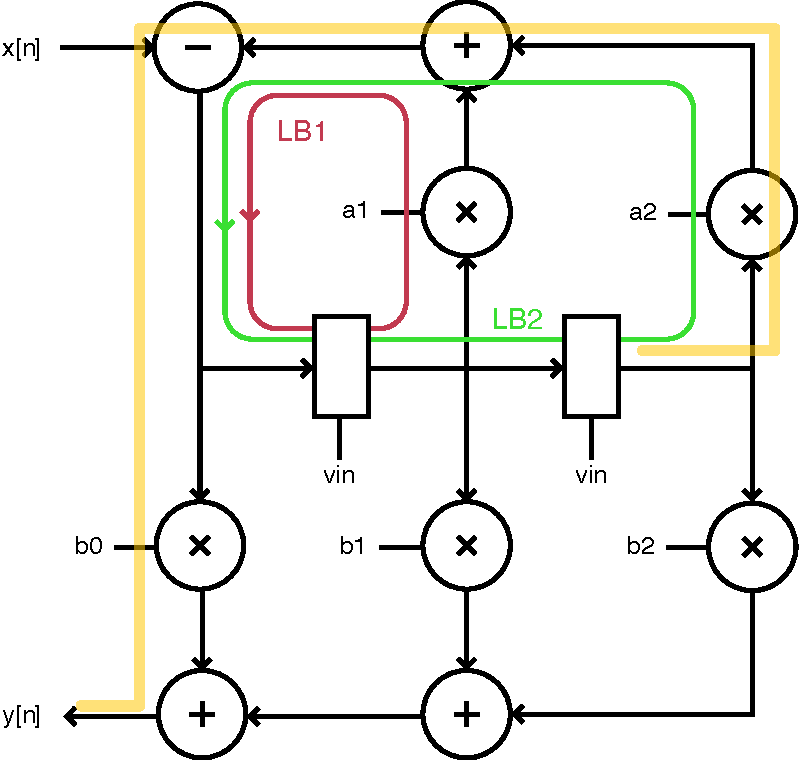
\includegraphics[width=0.4\linewidth]{./chapters/pictures/loop_bound_iir.pdf}
	\caption{Baseline IIR critical path}
	\label{fig:loop_bound_iir}
\end{figure}

In figure \ref{fig:loop_bound_iir} it is outlined in yellow the critical path of the non-optimized filter. If we define with
$T_{a}$ the delay of the adder and with with $T_{m}$ the delay of the multiplier, we obtain that

\begin{equation}
    \label{eq:baseline_iir_delay}
    CP_{iir} = 2T_{m} + 3T_{a}
\end{equation}

It can be also seen in the picture that there are two loops, namely $LB_{1}$ and $LB_{2}$. It is possible to calculate the
loop bound as follows:

\begin{align}\nonumber
    LB_{iir_{1}} = \frac{T_{m} + 2T_{a}}{1} \quad\quad LB_{iir_{2}} = \frac{T_{m} + 2T_{a}}{2}
\end{align}

Hence, we obtain

\begin{equation}\nonumber
    T_{iir_{\infty}} = \max \lbrace LB_{iir_{1}}, LB_{iir_{2}} \rbrace = LB_{iir_{1}} < CP_{iir}
\end{equation}

This means that a universal technique to improve the architecture exists; indeed pipelining could speed-up the architecture,
as there is a feed-forward cutset which divides the feed-forward multipliers from the upper part of the circuit. By placing
pipeline register there we obtain

\begin{equation}
    CP_{iir_{pipeline}} = T_{iir_{\infty}} = T_{m} + 2T_{a}
\end{equation}

This demonstrate that multiple optimization paths do exists for our architecture.

\subsection{Lookahead application}

The lookahead method works by recursively expanding the base equation. As the exercise stated that only one expansion was required,
we have proceeded in this way:

The equation of our filter is

\begin{equation}
    \label{eq:iir_eq}
    \begin{split}
        y[n] &= {\sum_{k=0}^{2} a_{k}y[n-k]} + {\sum_{i=0}^{2} b_{i}x[n-i]} = \\
        &= a_{0}y[n] + a_{1}y[n-1] + a_{2}y[n-2] + b_{0}x[n] + b_{1}x[n-1] + b_2[x-2]
    \end{split}
\end{equation}

We have calculated the formula of $y[n-1]$, which is

\begin{equation}
    \label{eq:yn-1}
    y[n-1] = a_{0}y[n-1] + a_{1}y[n-2] + a_{2}y[n-3] + b_{0}x[n-1] + b_{1}x[n-2] + b_2[x-3]
\end{equation}

If we insert \ref{eq:yn-1} in \ref{eq:iir_eq} the result is

\begin{equation}
    \label{eq:lookahead}
    \begin{split}
        y[n] &= a_{0}y[n] + a_{1}a_{0}y[n-1] + a^2_{1}y[n-2] + a_{1}a_{2}y[n-3] + a_{1}b_{0}x[n-1] + a_{1}b_{1}x[n-2]\ + \\
    & + a_{1}b_{2}x[n-3] + a_{2}y[n-2] + b_{0}x[n] + b_{1}x[n-1] + b_{2}x[n-2]
    \end{split}
\end{equation}

Which is our new filter's equation. Its block diagram is shown in figure \ref{fig:iir_lookahead}.

\begin{figure}[!ht]
	\centering
	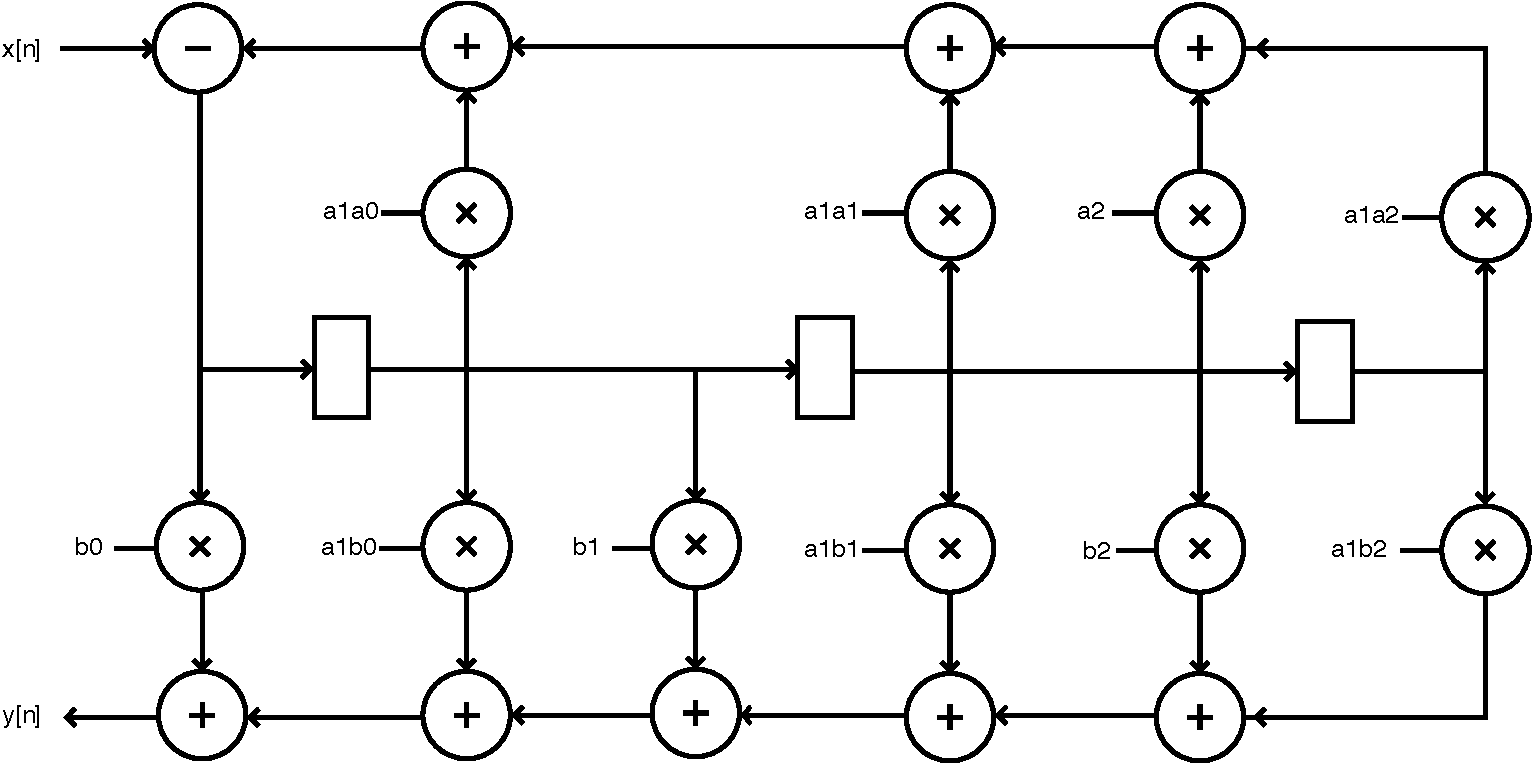
\includegraphics[width=0.7\linewidth]{./chapters/pictures/iir_lookahead.pdf}
	\caption{IIR lookahead}
	\label{fig:iir_lookahead}
\end{figure}

In equation \ref{eq:lookahead} it can be noticed that new coefficients appear in the form $a_{1}*a_{j}$ and $a_{1}*b_{j}$.
Their result does not fit in 12 bits, therefore we have decided to truncate them (by taking the 12 MSBs) to respect the original interface's bit width.

Starting from the structure shown in figure \ref{fig:iir_lookahead} we have derived a new C and VHDL model: the latter has been used as basis for the
optimizations described in section \ref{sec:iir_opt}, the former as golden model to check the results since, due to the new coefficients, the filter
has a different $THD$ and produces slightly different values. 

\section{Lookahead optimizations}
\label{sec:iir_opt}

Before applying any universal optimization technique, as always we needed to check if

$$T_{lookahead_{\infty}} < CP_{lookahead}$$

\begin{figure}[!ht]
	\centering
	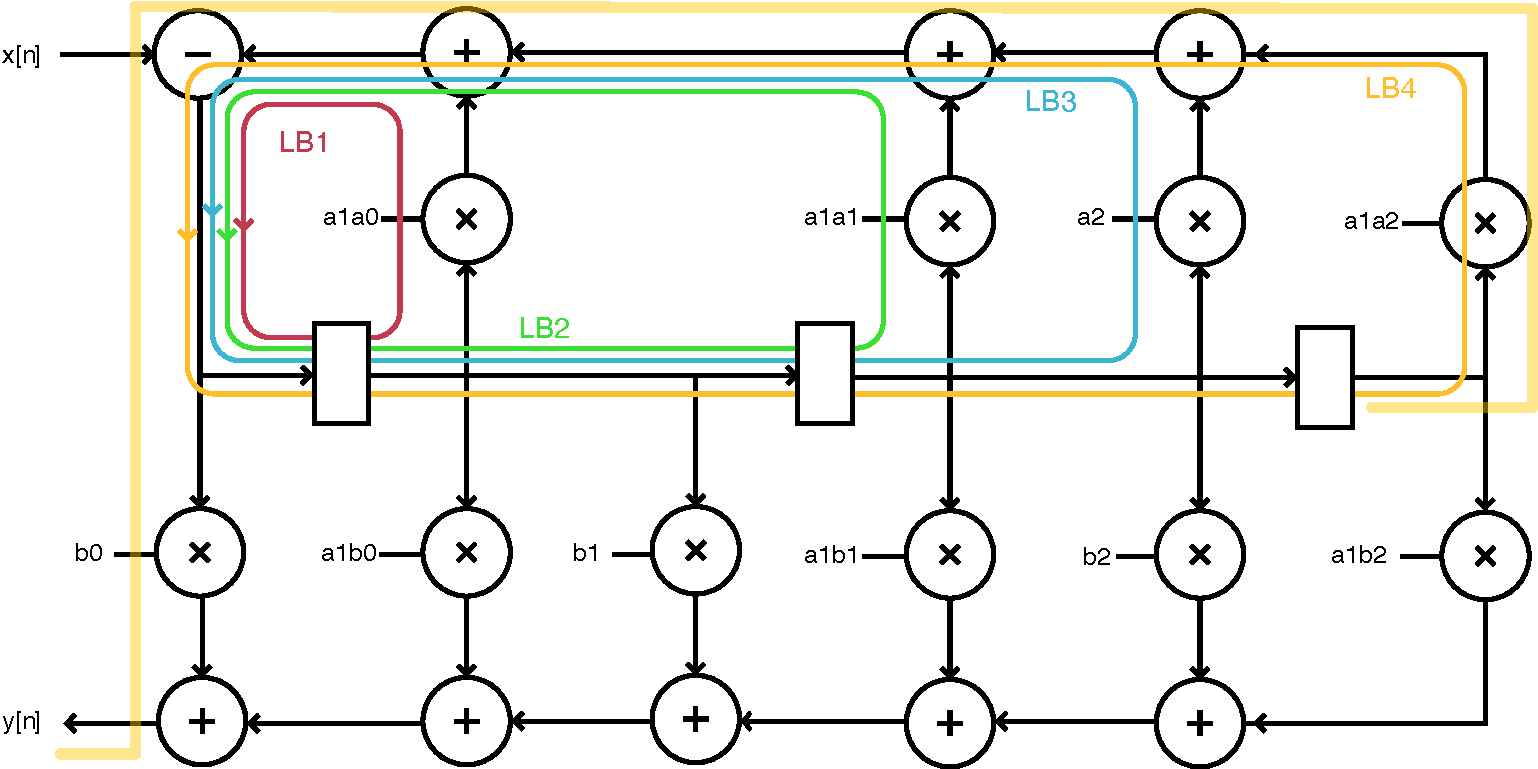
\includegraphics[width=0.7\linewidth]{./chapters/pictures/loop_bound_iir_lookahead.pdf}
	\caption{IIR lookahead critical path and loop bounds}
	\label{fig:lookahead_lb}
\end{figure}

In yellow it is highlighted the new critical path, which is equal to

\begin{equation}\nonumber
    \label{eq:lookahead_cp}
    CP_{lookahead} = 2T_{m} + 5T_{a}
\end{equation}

While in red, green, blue and orange are highlighted all the design's loops, which are respectively $LB_{1}$, $LB_{2}$, $LB_{3}$, $LB_{4}$ and are equal to

\begin{align}\nonumber
    &LB_{lookahead_{1}} = \frac{T_{m} + 2T_{a}}{1} &LB_{lookahead_{2}} = \frac{T_{m} + 3T_{a}}{2} \\ \nonumber
    &LB_{lookahead_{3}} = \frac{T_{m} + 4T_{a}}{2} &LB_{lookahead_{4}} = \frac{T_{m} + 4T_{a}}{3} \nonumber
\end{align}

Again, we have calculated $T_{lookahead_{\infty}}$ as

\begin{equation}\nonumber
    T_{lookahead_{\infty}} = \max \lbrace LB_{lookahead_{1}}, LB_{lookahead_{2}}, LB_{lookahead_{3}}, LB_{lookahead_{4}} \rbrace = LB_{lookahead_{1}}
\end{equation}

Which is smaller than $CP_{lookahead}$. To have $T_{lookahead_{\infty}} = CP_{lookahead}$ we have applied a combination of retiming and pipelining, as
shown in figure \ref{fig:lookahead_opt}.

\begin{figure}[!ht]
	\centering
	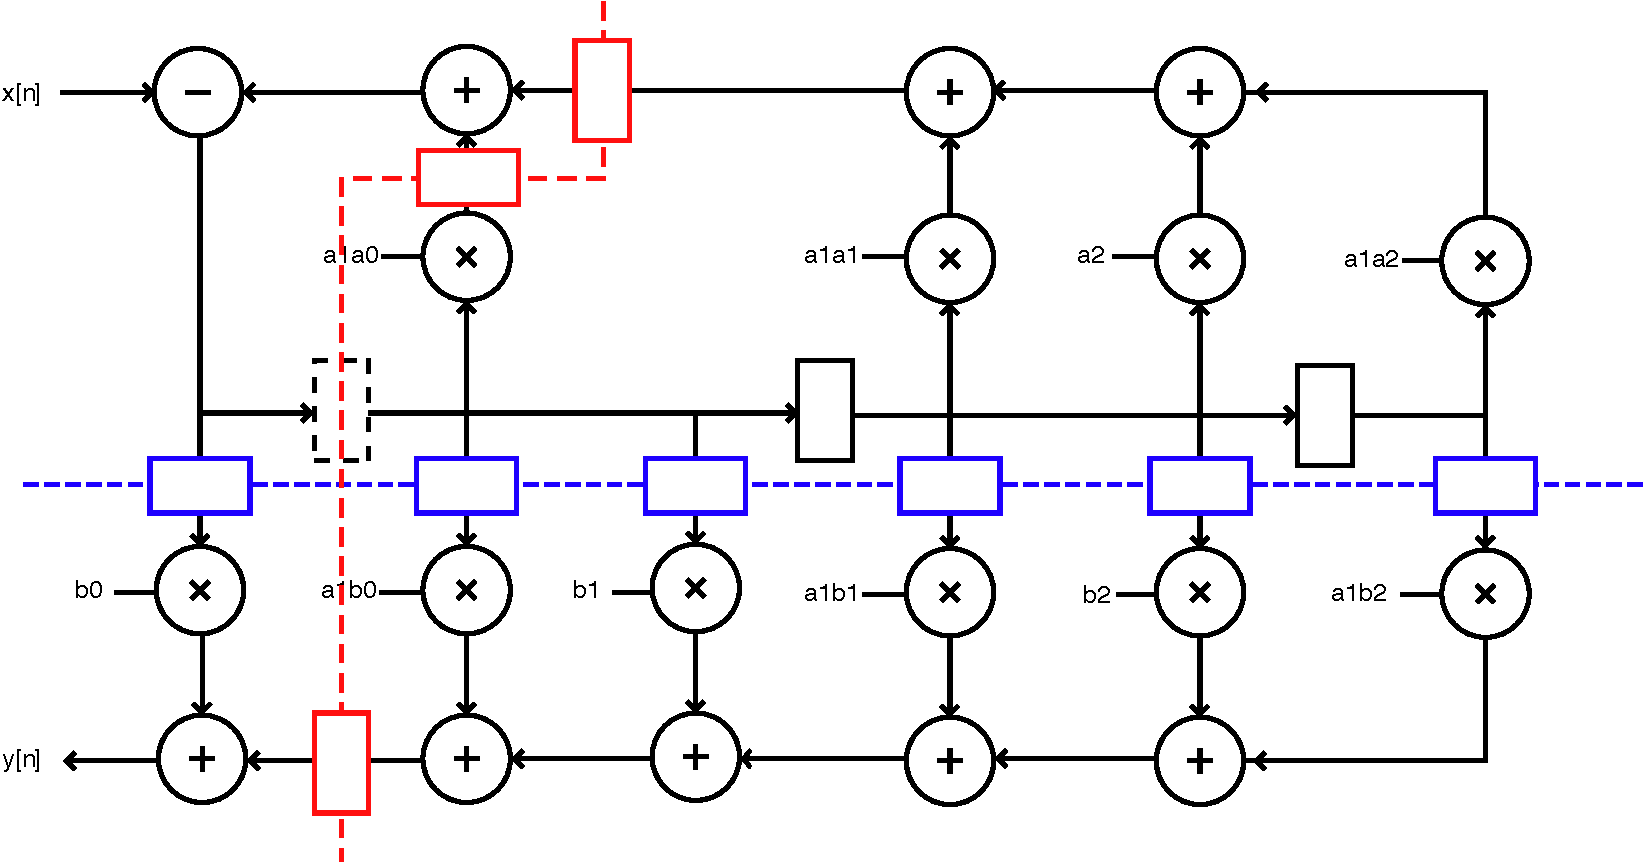
\includegraphics[width=0.8\linewidth]{./chapters/pictures/iir_opt.pdf}
	\caption{Optimized IIR lookahead}
	\label{fig:lookahead_opt}
\end{figure}

First, we applied retiming on the leftmost register, which is the dashed black one, by using the cutset shown in red. With the same color are shown the
retiming registers. Furthermore, in blue it is shown the forward cut-set used for pipelining and the related registers.
Pipelining, in respect to retiming, changes the behavior of the circuit. Indeed it had consequences on the delay of the $vin$ signal, which has been
adjusted accordingly. The new critical path has now a delay of

\begin{equation}
    CP_{lookahead} = T_{m} + 2T_{a}
\end{equation}

Which is better than the one of the baseline IIR described in equation \ref{eq:baseline_iir_delay}.
\section{Results comparison}
%%
%% NOW READ THE FILE master.tex  
\end{document}

